\section{Protegendo as Crianças: O Filtro AdGuard \faChild}

\noindent
Como garantir que seu filho não acesse sites adultos, de violência extrema ou de apostas no celular? Nós vamos colocar um filtro direto no \enquote{cano} de internet do aparelho.

\vspace{0.3cm} % Respiro
\begin{figure}[h]
	\centering
	\includegraphics[width=0.6\textwidth]{imagens/adguard_dns_dark.png}
	\caption*{(\citeauthor{adguard_dns} \citefield{adguard_dns}{version} - Versão oficial)}
\end{figure}

\vspace{0.3cm}
\noindent
Diferente de aplicativos espiões pesados, essa é uma configuração \enquote{escondida} no próprio sistema do seu celular (opção mais global que protege toda a sua navegação) ou navegador (opção mais direcionada que protege a navegação somente no navegador) que limpa a internet antes mesmo de ela aparecer na tela.

\vspace{0.3cm}
\noindent
Use os endereços fornecidos nos próximos passos ou obtenha-os diretamente da fonte pelo QR Code abaixo.

\vspace{0.3cm} % Respiro
\begin{center}
	\begin{minipage}{0.5\linewidth}
		\centering
		\textbf{\textcolor{AdguardDNSBlue}{\faAndroid \quad \faApple \quad \faDesktop}}\\[0.5cm]
		\href{https://bfaxke.short.gy/adguard-public-dns}{
			
\includegraphics[width=0.8\linewidth]{imagens/qr_adguard_public_dns.png}
		}\\[0.1cm]
		{\scriptsize (Toque ou escaneie)}
	\end{minipage}
\end{center}
\vspace{0.3cm} % Respiro após as imagens

\subsection*{Como configurar no Android:}

\noindent
Depois de ler com a câmera do seu dispositivo ou tocar no QR Code acima, você será direcionado para a página principal dos servidores de DNS públicos do AdGuard, assim como está mostrado no \enquote{Passo 1} abaixo. Mas atenção, como o objetivo aqui é economizar ao máximo o espaço físico no seu dispositivo, ignore a opção 1 por enquanto, então siga para a \enquote{Opção 2}, como indica o \enquote{Passo 2} seguinte:
\vspace{0.3cm}

% --- BLOCO DE IMAGENS 2 ---
\noindent
\begin{minipage}{\textwidth}
	\centering
	\begin{minipage}{0.45\textwidth}
		\centering
		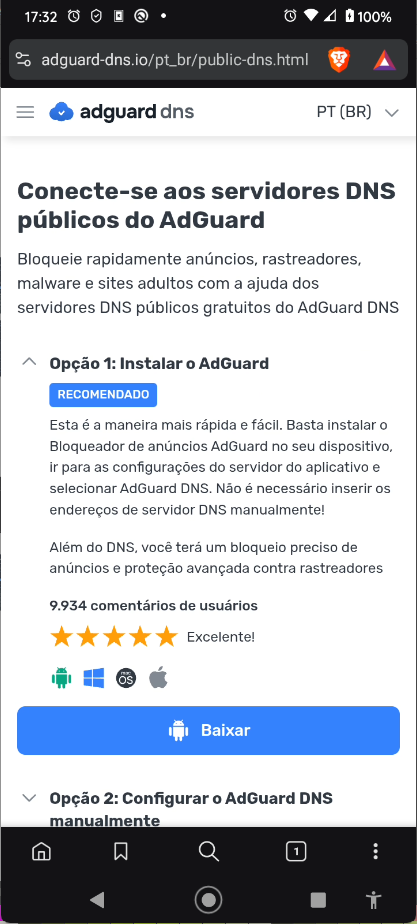
\includegraphics[trim={0cm 0cm 0cm 0cm}, clip, width=\textwidth]{imagens/adgard_dns_family_01.png}\\[0.2cm]
		\passo{AdguardDNSBlue}{1}{Nesta página, desça até a \enquote{Opção 2}}
	\end{minipage}
	\hfill
	\begin{minipage}{0.45\textwidth}
		\centering
		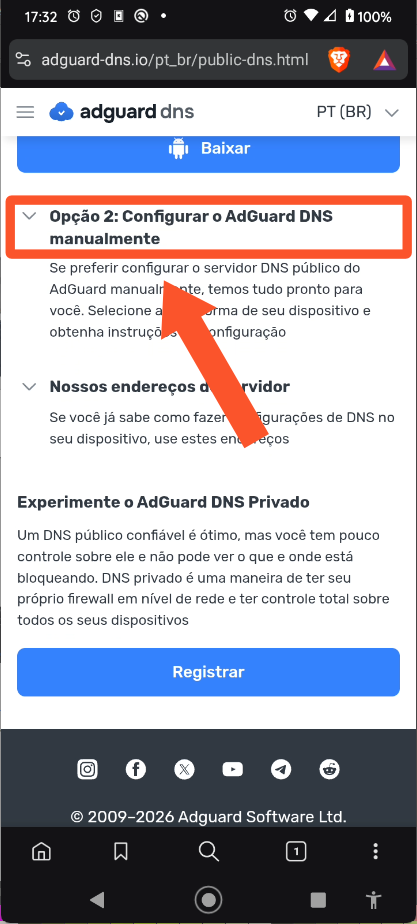
\includegraphics[trim={0cm 0cm 0cm 0cm}, clip, width=\textwidth]{imagens/adgard_dns_family_02.png}\\[0.2cm]
		\passo{AdguardDNSBlue}{2}{Toque em \enquote{Opção 2} \newline}
	\end{minipage}
\end{minipage}


\vspace{0.5cm}
\noindent
Se você seguiu as instruções acima e tocou na \enquote{Opção 2}, aparecerá a opção para o \enquote{Android}. Toque nela, como mostra no \enquote{Passo 3} a seguir, e role a tela para baixo até encontrar o item \textbf{\enquote{Servidor de proteção familiar}}, como mostra o \enquote{Passo 4}: 

\noindent
\begin{minipage}{\textwidth}
	\centering
	\begin{minipage}{0.45\textwidth}
		\centering
		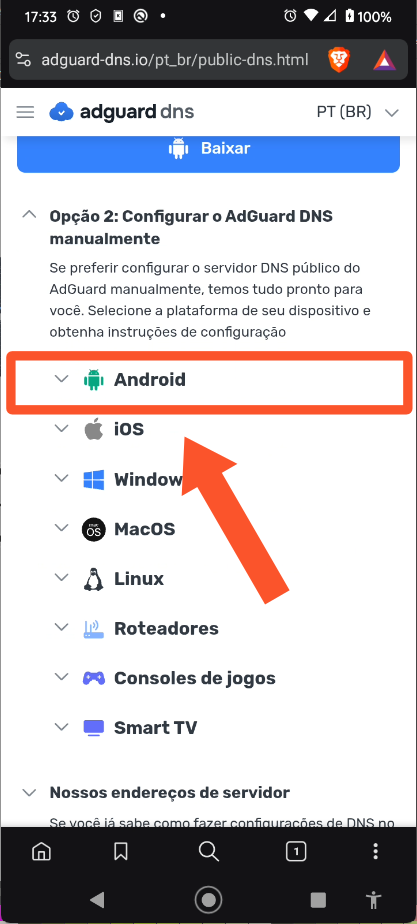
\includegraphics[trim={0cm 0cm 0cm 0cm}, clip, width=\textwidth]{imagens/adgard_dns_family_03.png}\\[0.2cm]
		\passo{AdguardDNSBlue}{3}{Toque em \enquote{Android} \newline} % CUIDADO!!!, essas linhas são para ajustar a altura da imagem nessa passo com a da imagem do passo anterior.
	\end{minipage}
	\hfill
	\begin{minipage}{0.45\textwidth}
		\centering
		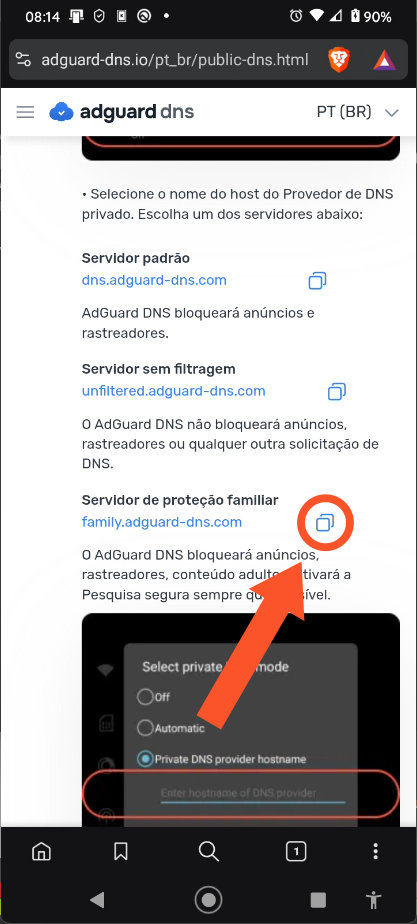
\includegraphics[trim={0cm 0cm 0cm 0cm}, clip, width=\textwidth]{imagens/adgard_dns_family_04.png}\\[0.2cm]
		\passo{AdguardDNSBlue}{4}{Toque na região indicada para copiar}
	\end{minipage}
\end{minipage}

\vspace{0.5cm}
\noindent
Apos ter copiado o endereço para a área de transferência, vamos para as configurações do seu dispositivo.

\vspace{0.3cm}
\noindent
Se a opção de configurar do seu dispositivo não estiver imediatamente acessível, você tem duas possíveis maneiras de acessá-la. A primeira é puxando duas vezes para baixo a barra superior onde mostra a hora e as notificações. Feito isso, no canto inferior esquerdo dela aparecerá o ícone da engrenagem, toque nele. A outra maneira é usar a pesquisa do Android para encontrar a palavra \enquote{Configurar} ou suas variações possíveis. Confira nos passos 3 e 4 abaixo essa duas maneiras, respectivamente: 

\vspace{0.3cm}

\noindent
\begin{minipage}{\textwidth}
	\centering
	\begin{minipage}{0.45\textwidth}
		\centering
		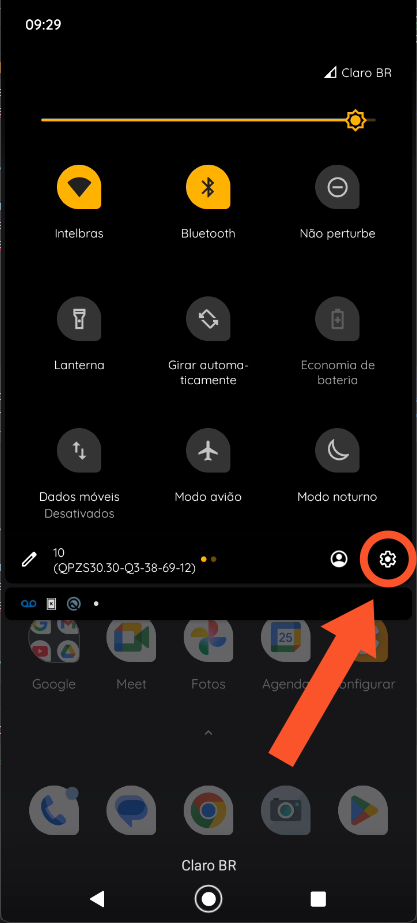
\includegraphics[trim={0cm 0cm 0cm 0cm}, clip, width=\textwidth]{imagens/adgard_dns_family_05.png}\\[0.2cm]
		\passo{AdguardDNSBlue}{5}{Toque na \enquote{Engrenagem} \newline} % CUIDADO!!!, essas linhas são para ajustar a altura da imagem nessa passo com a da imagem do passo anterior.
	\end{minipage}
	\hfill
	\begin{minipage}{0.45\textwidth}
		\centering
		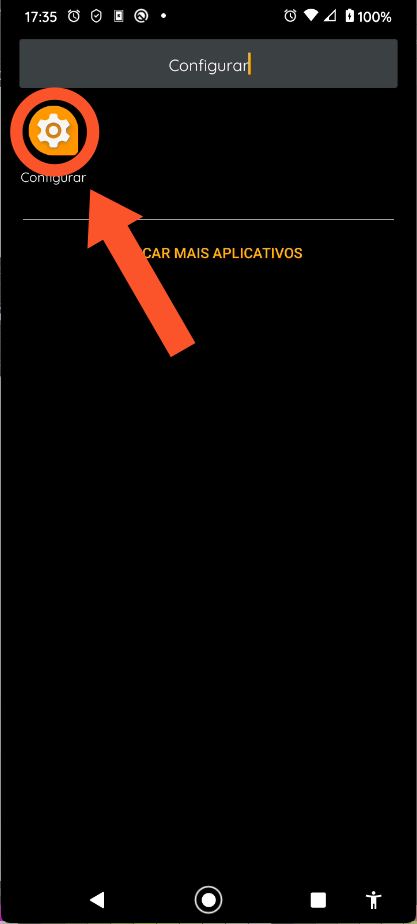
\includegraphics[trim={0cm 0cm 0cm 0cm}, clip, width=\textwidth]{imagens/adgard_dns_family_06.png}\\[0.2cm]
		\passo{AdguardDNSBlue}{6}{Toque em \enquote{Configurar}}
	\end{minipage}
\end{minipage}
\vspace{0.3cm}

\noindent
Efetuados os passos anteriores, toque em \enquote{Pesquisar configurações} (\textbf{Passo 5}) e digite \enquote{DNS} (\textbf{Passo 6}), ou \enquote{DNS particular}, ou suas possíveis variações. Acompanhe abaixo:

\vspace{0.3cm}
\noindent
\begin{minipage}{\textwidth}
	\centering
	\begin{minipage}{0.45\textwidth}
		\centering
		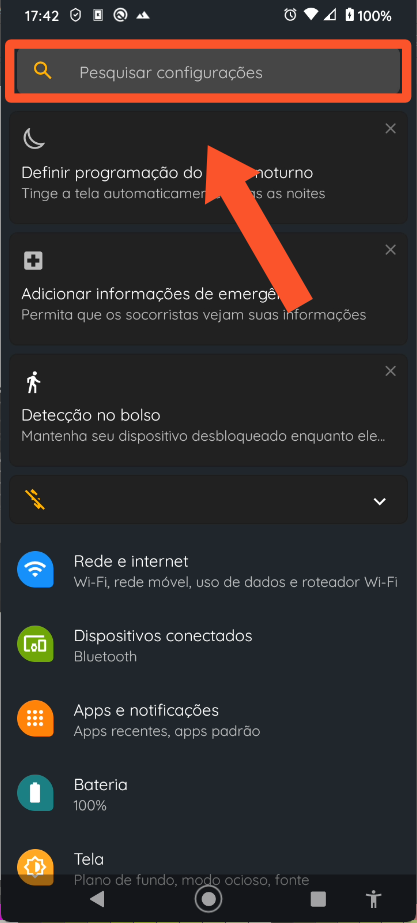
\includegraphics[trim={0cm 0cm 0cm 0cm}, clip, width=\textwidth]{imagens/adgard_dns_family_07.png}\\[0.2cm]
		\passo{AdguardDNSBlue}{7}{Toque em \enquote{Pesquisar configurações}}
	\end{minipage}
	\hfill
	\begin{minipage}{0.45\textwidth}
		\centering
		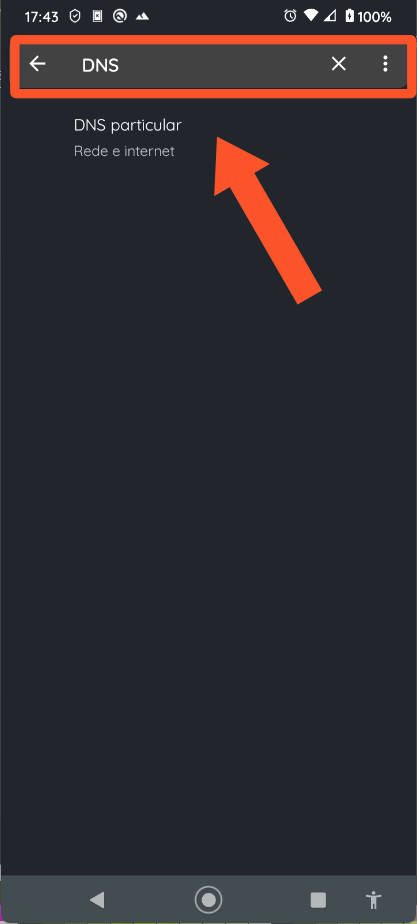
\includegraphics[trim={0cm 0cm 0cm 0cm}, clip, width=\textwidth]{imagens/adgard_dns_family_08.png}\\[0.2cm]
		\passo{AdguardDNSBlue}{8}{Digite \enquote{DNS} \newline} % CUIDADO!!!, essas linhas são para ajustar a altura da imagem nessa passo com a da imagem do passo anterior.
	\end{minipage}
\end{minipage}
\vspace{0.3cm}

\noindent
O \textbf{Passo 6} nos mostra onde se encontram as configurações de DNS do nosso dispositivo. Não vamos procurar mais, então, basta tocar em \enquote{DNS particular} para acessar as configurações do DNS. Veja abaixo:

\vspace{0.3cm}
\noindent
\begin{minipage}{\textwidth}
	\centering
	\begin{minipage}{0.45\textwidth}
		\centering
		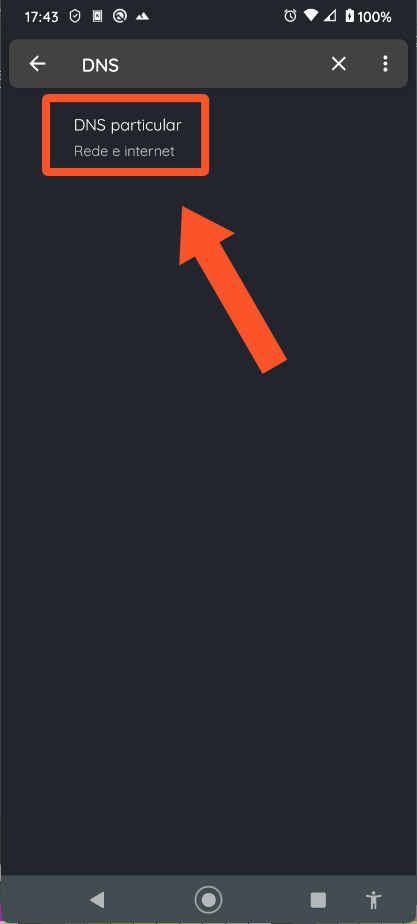
\includegraphics[trim={0cm 0cm 0cm 0cm}, clip, width=\textwidth]{imagens/adgard_dns_family_09.png}\\[0.2cm]
		\passo{AdguardDNSBlue}{9}{Toque em \enquote{DNS particular}}
	\end{minipage}
	\hfill
	\begin{minipage}{0.45\textwidth}
		\centering
		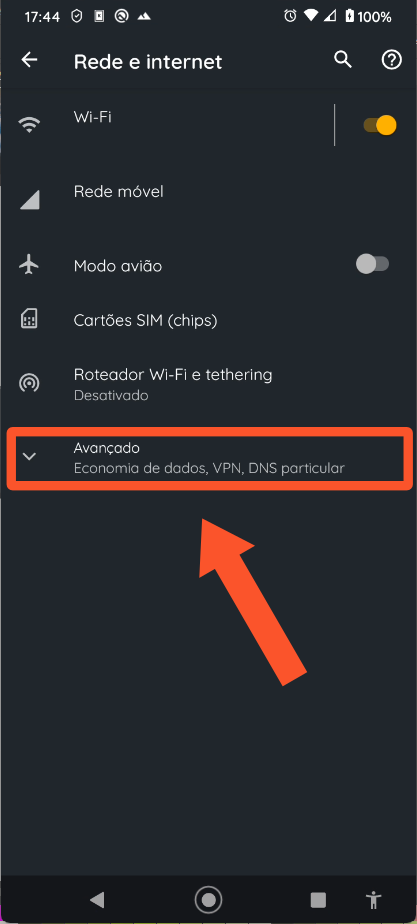
\includegraphics[trim={0cm 0cm 0cm 0cm}, clip, width=\textwidth]{imagens/adgard_dns_family_10.png}\\[0.2cm]
		\passo{AdguardDNSBlue}{10}{Toque em \enquote{Avançado}}
	\end{minipage}
\end{minipage}
\vspace{0.3cm}

\noindent
Estamos quase lá. Lembre-se que já copiamos o endereço do servidor público AdGuard DNS Family no \textbf{Passo 4:}

\vspace{0.3cm}
% Caixa isolada para facilitar a cópia no celular
\noindent
\begin{center}
	\begin{tcolorbox}[
		colback=NordBackground, 
		colframe=AdguardDNSBlue, 
		width=0.8\linewidth, 
		halign=center,       % Centraliza horizontalmente
		valign=center,       % Centraliza verticalmente
		boxrule=1pt, 
		arc=2mm,
		top=3mm,             % Ajuste fino da margem superior
		bottom=3mm           % Ajuste fino da margem inferior
		]
		\Large \sffamily \textbf{\textcolor{AdguardDNSBlue}{family.adguard-dns.com}}
	\end{tcolorbox}
	{\scriptsize (Selecione e copie)}
\end{center}
\vspace{0.3cm}

\noindent
Se você não lembra, copie/anote o endereço acima (exatamente como está, tudo minúsculo), ou retorne ao \textbf{Passo 4} e copie o endereço. Depois disso, e após ter realizado o \textbf{Passo 10}, aparecerá a opção procurada, ou seja: \textbf{DNS particular}, toque nela. Acompanhe isso nas imagens abaixo:

\vspace{0.3cm}
\noindent
\begin{minipage}{\textwidth}
	\centering
	\begin{minipage}{0.45\textwidth}
		\centering
		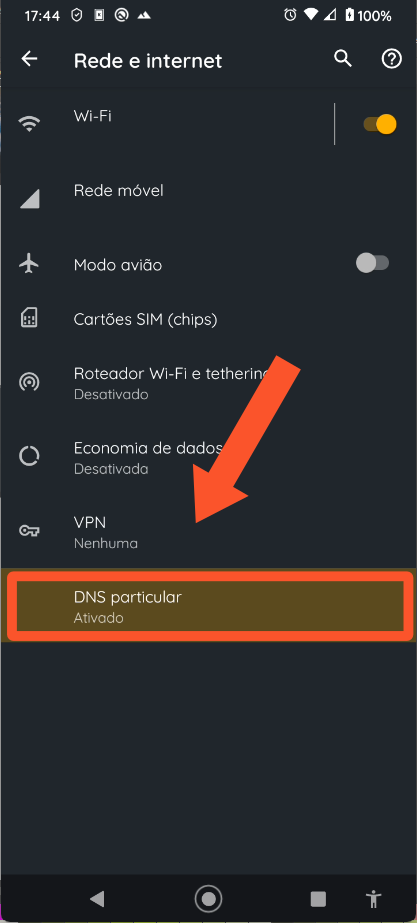
\includegraphics[trim={0cm 0cm 0cm 0cm}, clip, width=\textwidth]{imagens/adgard_dns_family_11.png}\\[0.2cm]
		\passo{AdguardDNSBlue}{11}{Toque em \enquote{DNS particular}} \newline
	\end{minipage}
	\hfill
	\begin{minipage}{0.45\textwidth}
		\centering
		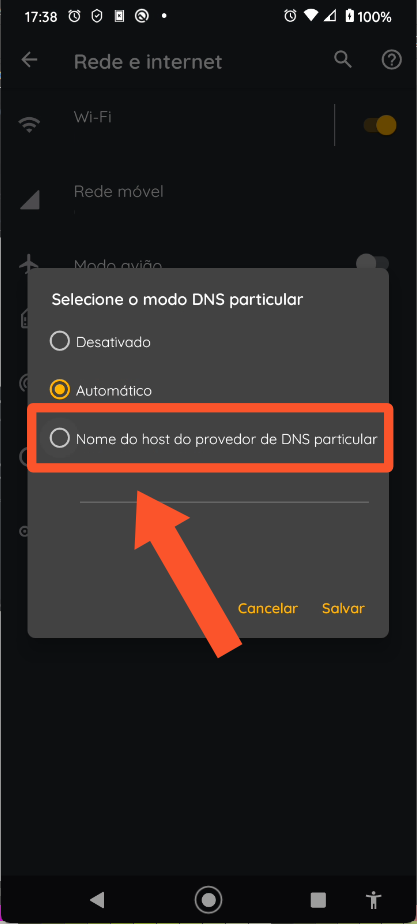
\includegraphics[trim={0cm 0cm 0cm 0cm}, clip, width=\textwidth]{imagens/adgard_dns_family_12.png}\\[0.2cm]
		\passo{AdguardDNSBlue}{12}{Toque em \enquote{Nome do host do provedor de DNS particular}}
	\end{minipage}
\end{minipage}
\vspace{0.3cm}

\noindent
Como o \textbf{Passo 12} realizado, ficara disponível um campo para adicionar o DNS AdGuard Family. Veja a seguir:

\vspace{0.3cm}
\noindent
\begin{minipage}{\textwidth}
	\centering
	\begin{minipage}{0.45\textwidth}
		\centering
		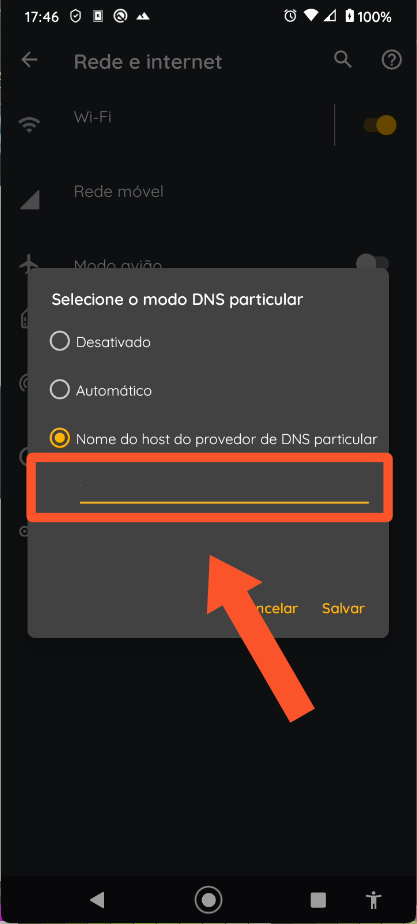
\includegraphics[trim={0cm 0cm 0cm 0cm}, clip, width=\textwidth]{imagens/adgard_dns_family_13.png}\\[0.2cm]
		\passo{AdguardDNSBlue}{13}{Digite ou cole o \enquote{Nome do host de DNS} no campo vazio}
	\end{minipage}
	\hfill
	\begin{minipage}{0.45\textwidth}
		\centering
		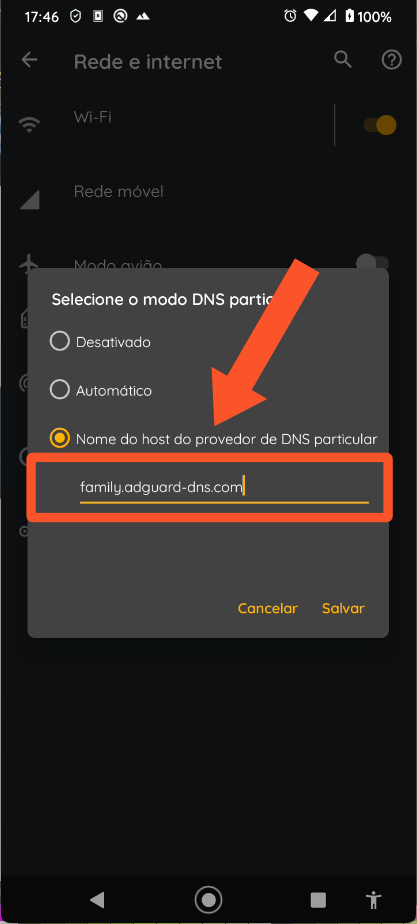
\includegraphics[trim={0cm 0cm 0cm 0cm}, clip, width=\textwidth]{imagens/adgard_dns_family_14.png}\\[0.2cm]
		\passo{AdguardDNSBlue}{14}{Desta forma} \newline
	\end{minipage}
\end{minipage}
\vspace{0.3cm}

\noindent
Feito isso, agora você pode salvar que o DNS será aplicado no seu Android. Veja como deve ficar nos passos seguintes:

\vspace{0.3cm}
\noindent
\begin{minipage}{\textwidth}
	\centering
	\begin{minipage}{0.45\textwidth}
		\centering
		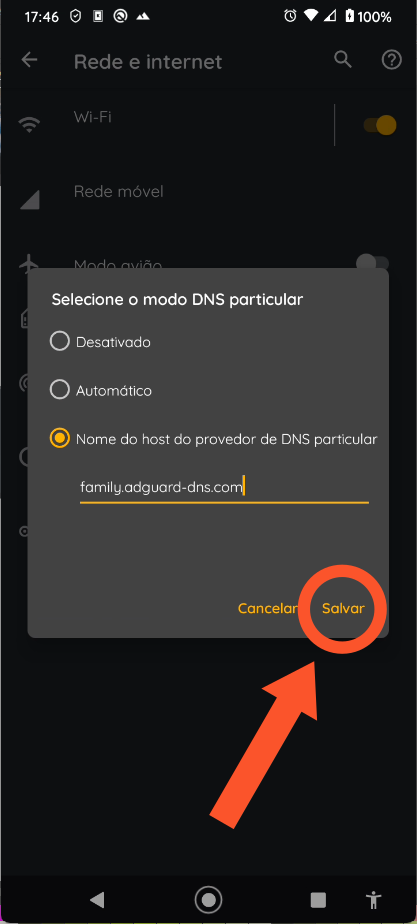
\includegraphics[trim={0cm 0cm 0cm 0cm}, clip, width=\textwidth]{imagens/adgard_dns_family_15.png}\\[0.2cm]
		\passo{AdguardDNSBlue}{15}{Toque em \enquote{Salvar}}
	\end{minipage}
	\hfill
	\begin{minipage}{0.45\textwidth}
		\centering
		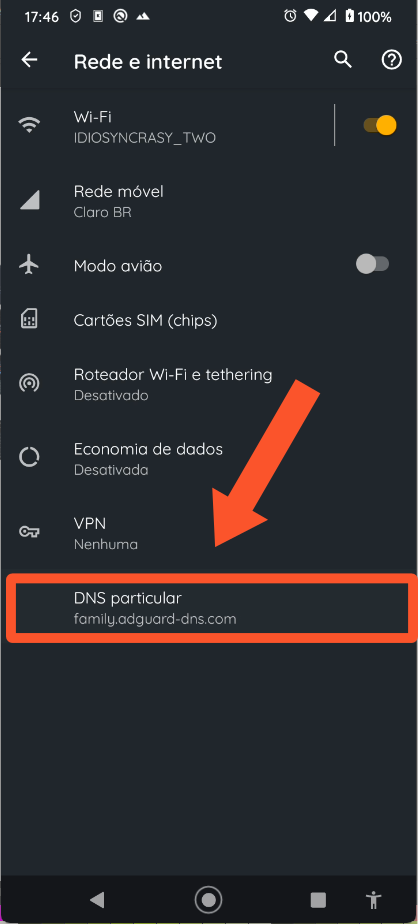
\includegraphics[trim={0cm 0cm 0cm 0cm}, clip, width=\textwidth]{imagens/adgard_dns_family_16.png}\\[0.2cm]
		\passo{AdguardDNSBlue}{16}{Pronto!}
	\end{minipage}
\end{minipage}
\vspace{0.3cm}

\subsection*{Como configurar no iOS:}

\noindent
Para realizar essa configuração no iOS, você precisa baixar ou criar um perfil de configuração. Para isso, vá até a página do \textbf{Passo 1} e escolha um servidor DNS entre os disponíveis e siga o passo a passo indicado nas instruções. 

\newpage
\subsection*{Como configurar diretamente no Navegador:}

\noindent
Vamos usar aqui o navegador Brave, mas, feitas as devidas adaptações, pode ser em qualquer navegador de sua preferência. A ideia aqui é segmentar de forma direcional a filtragem para um navegador específico.
\vspace{0.3cm} % Respiro após as imagens

\vspace{0.3cm}
\noindent
Como na configuração anterior, use os próximo QR Code ou simplesmente copie/anote o endereço do servidor de proteção familiar mais abaixo:

\vspace{0.3cm} % Respiro
\noindent
\begin{center}
	\begin{minipage}{0.5\linewidth}
		\centering
		\textbf{\textcolor{AdguardDNSBlue}{\faAndroid \quad \faApple \quad \faDesktop}}\\[0.5cm]
		\href{https://bfaxke.short.gy/adguard-public-dns}{
			
\includegraphics[width=0.8\linewidth]{imagens/qr_adguard_public_dns.png}
		}\\[0.1cm]
		{\scriptsize (Toque ou escaneie)}
	\end{minipage}
\end{center}
\vspace{0.3cm}


% Caixa isolada para facilitar a cópia no celular
\noindent
\begin{center}
	\begin{tcolorbox}[
		colback=NordBackground, 
		colframe=AdguardDNSBlue, 
		width=1\linewidth, 
		halign=center,       % Centraliza horizontalmente
		valign=center,       % Centraliza verticalmente
		boxrule=1pt, 
		arc=2mm,
		top=3mm,             % Ajuste fino da margem superior
		bottom=3mm,           % Ajuste fino da margem inferior
		left=5mm,
		right=5mm
		]
		\Large \sffamily \textbf{\textcolor{AdguardDNSBlue}{https://family.adguard-dns.com/dns-query}}
	\end{tcolorbox}
	{\scriptsize (Selecione e copie)}
\end{center}
\vspace{0.3cm}

\noindent
Acesse a página fornecida pelo QR Code anterior, mas se você preferiu copiar o endereço, abra seu navegador e avance direto para o \textbf{Passo 6}.

\vspace{0.3cm}
\noindent
Acessando o endereço do QR Code no navegador Brave, a página fica como no \textbf{Passo 1} da imagem abaixo onde você vai percorrer a página para baixo até encontrar o campo \enquote{Nossos endereços de servidor}:

\vspace{0.3cm}
\noindent
\begin{minipage}{\textwidth}
	\centering
	\begin{minipage}{0.45\textwidth}
		\centering
		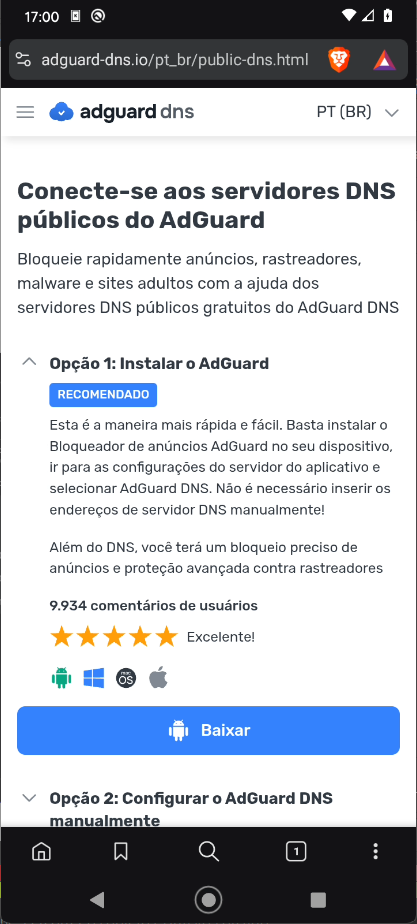
\includegraphics[trim={0cm 0cm 0cm 0cm}, clip, width=\textwidth]{imagens/adgard_dns_family_17.png}\\[0.2cm]
		\passo{AdguardDNSBlue}{1}{Suba está página até o campo \enquote{Nossos endereços de servidor}}
	\end{minipage}
	\hfill
	\begin{minipage}{0.45\textwidth}
		\centering
		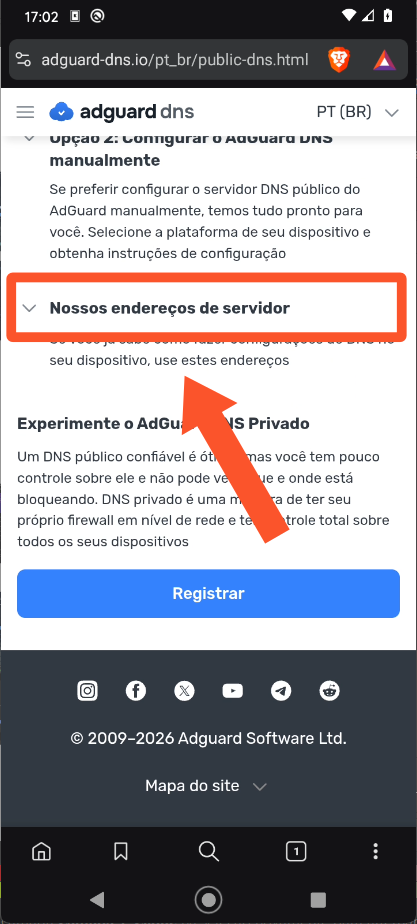
\includegraphics[trim={0cm 0cm 0cm 0cm}, clip, width=\textwidth]{imagens/adgard_dns_family_18.png}\\[0.2cm]
		\passo{AdguardDNSBlue}{2}{Toque em \enquote{Nossos endereços de servidor}}
	\end{minipage}
\end{minipage}
\vspace{0.3cm}

\noindent
Nos passos abaixo, você deve tocar no campo \enquote{DNS-over-HTTPS} (\textbf{Passo 3}) para abir as opções de servidores. No campo \enquote{Servido de proteção familiar} (\textbf{Passo 4}) toque no ícone copiar no canto inferior direito. Após copiado o endereço, siga para os passo seguintes.

\vspace{0.3cm}
\noindent
\begin{minipage}{\textwidth}
	\centering
	\begin{minipage}{0.45\textwidth}
		\centering
		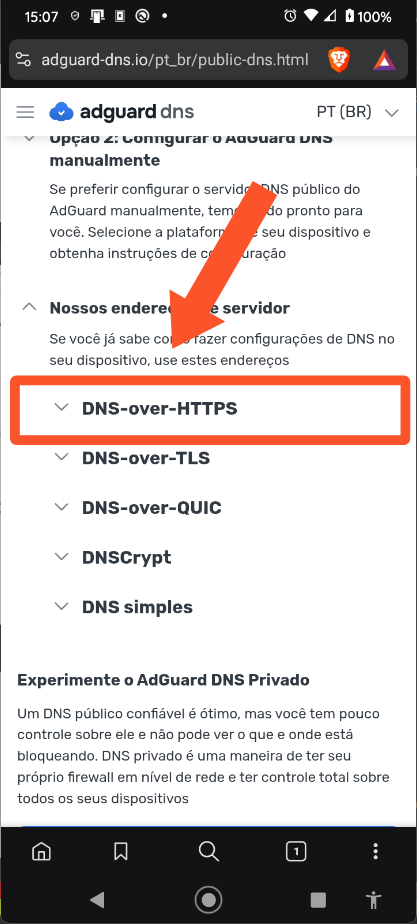
\includegraphics[trim={0cm 0cm 0cm 0cm}, clip, width=\textwidth]{imagens/adgard_dns_family_19.png}\\[0.2cm]
		\passo{AdguardDNSBlue}{3}{Toque em \enquote{DNS-over-HTTPS}}
	\end{minipage}
	\hfill
	\begin{minipage}{0.45\textwidth}
		\centering
		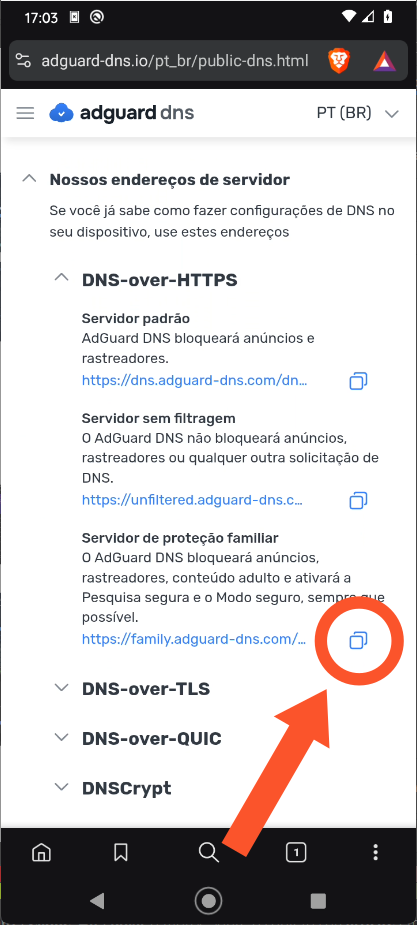
\includegraphics[trim={0cm 0cm 0cm 0cm}, clip, width=\textwidth]{imagens/adgard_dns_family_20.png}\\[0.2cm]
		\passo{AdguardDNSBlue}{4}{Toque em \enquote{Nossos endereços de servidor}}
	\end{minipage}
\end{minipage}
\vspace{0.3cm}

\noindent
Nos próximos passos, vamos acessar as configurações do navegador. Note no \textbf{Passo 5} que o ícone de copiar foi substituído pelo ícone de visto. Além, é claro, da mensagem no botão azul abaixo da seta avisando que a ação foi efetuada com sucesso. Já no \textbf{Passo 6}, você deve tocar nos três pontinho na vertical como indicado abaixo:

\vspace{0.3cm}
\noindent
\begin{minipage}{\textwidth}
	\centering
	\begin{minipage}{0.45\textwidth}
		\centering
		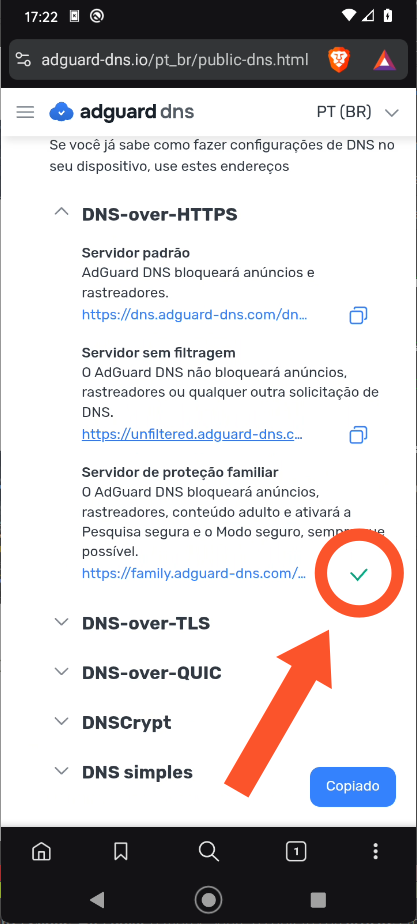
\includegraphics[trim={0cm 0cm 0cm 0cm}, clip, width=\textwidth]{imagens/adgard_dns_family_21.png}\\[0.2cm]
		\passo{AdguardDNSBlue}{5}{Ótimo, \enquote{Copiado}} \newline % O comando \newline ajusta altura da base dessa imagem com a imagem seguinte
	\end{minipage}
	\hfill
	\begin{minipage}{0.45\textwidth}
		\centering
		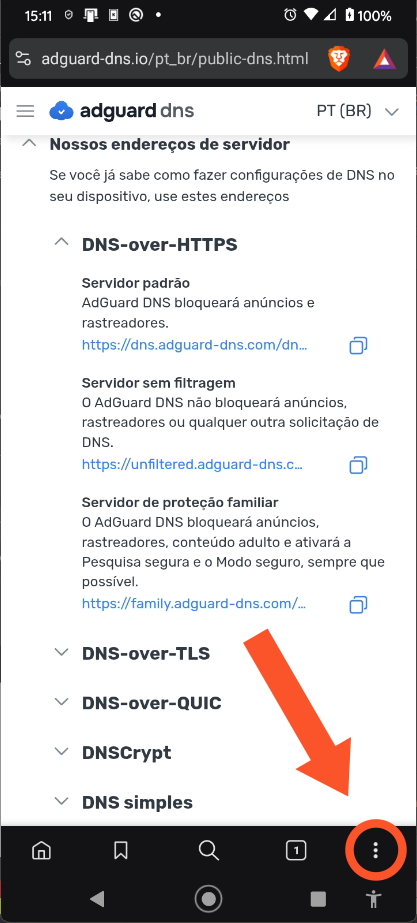
\includegraphics[trim={0cm 0cm 0cm 0cm}, clip, width=\textwidth]{imagens/adgard_dns_family_22.png}\\[0.2cm]
		\passo{AdguardDNSBlue}{6}{Toque nos três pontos dispostos na vertical}
	\end{minipage}
\end{minipage}
\vspace{0.3cm}

\noindent
Ótimo! Agora estamos quase lá. Ao tocar nos três pontos dispostos na vertical, o Brave, abrirá um menu de contexto (não tenho certeza se denomino assim mesmo). Percorra ele até encontrar as configurações (\textbf{Passo 7}). 

\vspace{0.3cm}
\noindent
\begin{minipage}{\textwidth}
	\centering
	\begin{minipage}{0.45\textwidth}
		\centering
		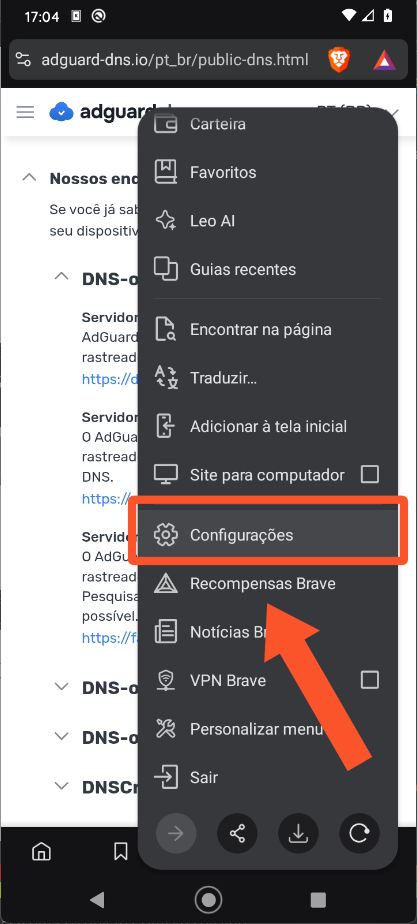
\includegraphics[trim={0cm 0cm 0cm 0cm}, clip, width=\textwidth]{imagens/adgard_dns_family_23.png}\\[0.2cm]
		\passo{AdguardDNSBlue}{7}{Toque em \enquote{Configurações}} \newline % O comando \newline ajusta altura da base dessa imagem com a imagem seguinte
	\end{minipage}
	\hfill
	\begin{minipage}{0.45\textwidth}
		\centering
		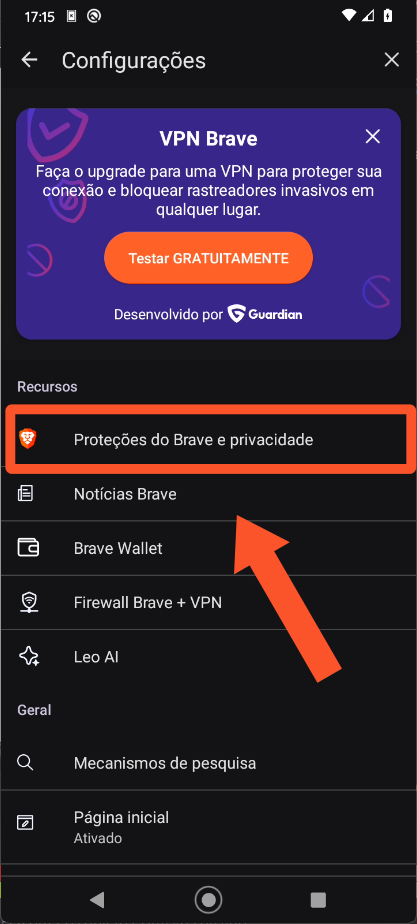
\includegraphics[trim={0cm 0cm 0cm 0cm}, clip, width=\textwidth]{imagens/adgard_dns_family_24.png}\\[0.2cm]
		\passo{AdguardDNSBlue}{8}{Toque em \enquote{Proteções do Brave e privacidade}}
	\end{minipage}
\end{minipage}
\vspace{0.3cm}

\vspace{0.5cm}
\begin{tcolorbox}[colback=NordBackground, colframe=AdguardGreen, title=\faCheckCircle\ Vantagem Extra]
	\textcolor{white}{Além de proteger as crianças contra sites perigosos, este filtro também bloqueia boa parte das propagandas em jogos e aplicativos gratuitos!}
\end{tcolorbox}